% Compiler ce document 

% package de base
\documentclass[10pt,a4paper]{article}
\usepackage[utf8]{inputenc}
\usepackage{listings}

% langues
\usepackage[usenames,dvipsnames]{xcolor}
\usepackage[francais]{babel}
\usepackage[T1]{fontenc}
\usepackage{amsmath}
\usepackage{amsfonts}
\usepackage{amssymb}
\usepackage{graphicx}
\usepackage{tabularx}
\usepackage{colortbl}
\usepackage[hidelinks]{hyperref} % liens
\usepackage{fancyhdr} % En tetes / bas de page
\usepackage{helvet} % police helvetica
\usepackage[hidelinks]{hyperref}
\usepackage{xcolor} % Style pour affichage du C
\usepackage{courier} % police pour les listings
\usepackage{tikz}

\usepackage{listingsutf8}

% Page de Garde -- Necessite d'installer le package titling, si probleme
% commenter la ligne suivante ainsi que les infos necessaires a la page
% de garde
\usepackage{pageGarde/Garde_perso}

% commande pour faire des sections sans nombre 
% tout en la rajoutant dans la table des matières
\newcommand\sectionWithoutNumber[1]{\section*{#1} \addcontentsline{toc}{section}{\protect\numberline{}#1}}
\newcommand\subsectionWithoutNumber[1]{\subsection*{#1} \addcontentsline{toc}{subsection}{\protect\numberline{}#1}}
\newcommand\subsubsectionWithoutNumber[1]{\subsection*{#1} \addcontentsline{toc}{subsubsection}{\protect\numberline{}#1}}
% définition de nouvelles couleurs
\definecolor{lightblue}{rgb}{0.8,0.8,0.9}
\definecolor{grossblue}{rgb}{0,0,0.7}
%marge des pages
\setlength{\textwidth}{16cm}
\setlength{\textheight}{24cm}
\setlength{\oddsidemargin}{0cm}
\setlength{\voffset}{-1.5cm}
\setlength{\headheight}{15pt}

% set la police en arial
%% Sans-serif Arial-like fonts
\renewcommand{\rmdefault}{phv} 
\renewcommand{\sfdefault}{phv} 
\usepackage{tabularx}
\usepackage{graphicx}
\usepackage{eurosym}
\usepackage{xspace}
\newcommand{\projectname}[0]{LTANR\xspace} 

% configuration pour des listings
\lstset{ 
  showspaces=false,      
  showstringspaces=false, 
  showtabs=false,               
  tabsize=3,                     
  numbers=left
}

%enlève indentation en début de paragraphe
\setlength\parindent{0pt}

%style de l'en-tête de page
\pagestyle{fancy}

% style pour code en c
\lstdefinestyle{customc}{
  belowcaptionskip=1\baselineskip,
  breaklines=true,
  frame=L,
  xleftmargin=\parindent,
  language=C,
  showstringspaces=false,
  basicstyle=\scriptsize\ttfamily,
  keywordstyle=\bfseries\color{green!40!black},
  commentstyle=\itshape\color{purple!40!black},
  identifierstyle=\color{blue},
  stringstyle=\color{orange},
}

\lstdefinelanguage{VHDL}{
      morekeywords=[1]{
        library,use,all,entity,is,port,in,out,end,architecture,of,
        begin,and,or,Not,downto,ALL
      },
      morekeywords=[2]{
        STD_LOGIC_VECTOR,STD_LOGIC,IEEE,STD_LOGIC_1164,
        NUMERIC_STD,STD_LOGIC_ARITH,STD_LOGIC_UNSIGNED,std_logic_vector,
        std_logic
      },
      morecomment=[l]--
    }
    \usepackage[usenames,dvipsnames]{xcolor}
    \colorlet{keyword}{blue!100!black!80}
    \colorlet{STD}{Lavender}
    \colorlet{comment}{green!80!black!90}
    \lstdefinestyle{vhdl}{
      language     = VHDL,
      basicstyle   = \footnotesize \ttfamily,
      keywordstyle = [1]\color{keyword}\bfseries,
      keywordstyle = [2]\color{STD}\bfseries,
      commentstyle = \color{comment}
      breaklines=true,                % sets automatic line breaking
      tabsize=3                                % sets default tabsize to 2 spaces
    }

\lstset{escapechar=@,style=customc}
\lstset{inputencoding=utf8/latin1} %affiche les accents dans le listing

% Mise en forme de la page de titre
\author{João Miguel Domingues Pedrosa\\Rick Wertenbroek}
\title{Mémoire cache}
\dest{}

% Informations necessaires a la page de garde
% Commenter si probleme de compilation
\acro{CSF}
\matter{Conception de système numérique sur FPGA}
\date{\today}

%en-tête
\lhead{Domingues \& Wertenbroek}
\chead{Mémoire cache}
\rhead{\theAcro}

%pied-de-page
\lfoot{HEIG-VD}
\cfoot{\today}
\rfoot{\thepage}

\begin{document}
\maketitle
\newpage
\tableofcontents
\newpage

%Ici commence réelement l'écriture du rapport
\section{Introduction}
Pour ce laboratoire, nous avons dû implémenter une mémoire cache interne à une FPGA. La mémoire cache sert à accélérer les accès en mémoire en allant chercher les données dans une zone mémoire plus petit mais plus proche donc plus rapide. Il faut donc interface, avec un simple bus, les accès entre l'utilisateur (agent) et la mémoire externe (DDR).

\section{Mémoire Cache}
\subsection{Mémoire}
La mémoire se sépare en plusieurs attributs qui sont les suivants:\\

\begin{itemize}
	\item Data (vecteur): il s'agit des données
	\item Tag  (vecteur): permet de vérifier si le bloque mémoire rechercher est juste
	\item Valid (bit): indique si la ligne en cache est initialisé
	\item Dirty (bit): indique si il y a eu un accès écriture dans la ligne\\
\end{itemize}

Pour chaque attributs, nous avons un tableau de la taille du nombre de ligne en cache que l'on accédera grâce à l'index retrouvé par l'adresse rechercher par l'agent.

\newpage

\subsection{Contrôleur}
Pour représenter le fonctionnement de la cache, nous sommes parties d'une machine d'état.

\begin{center}

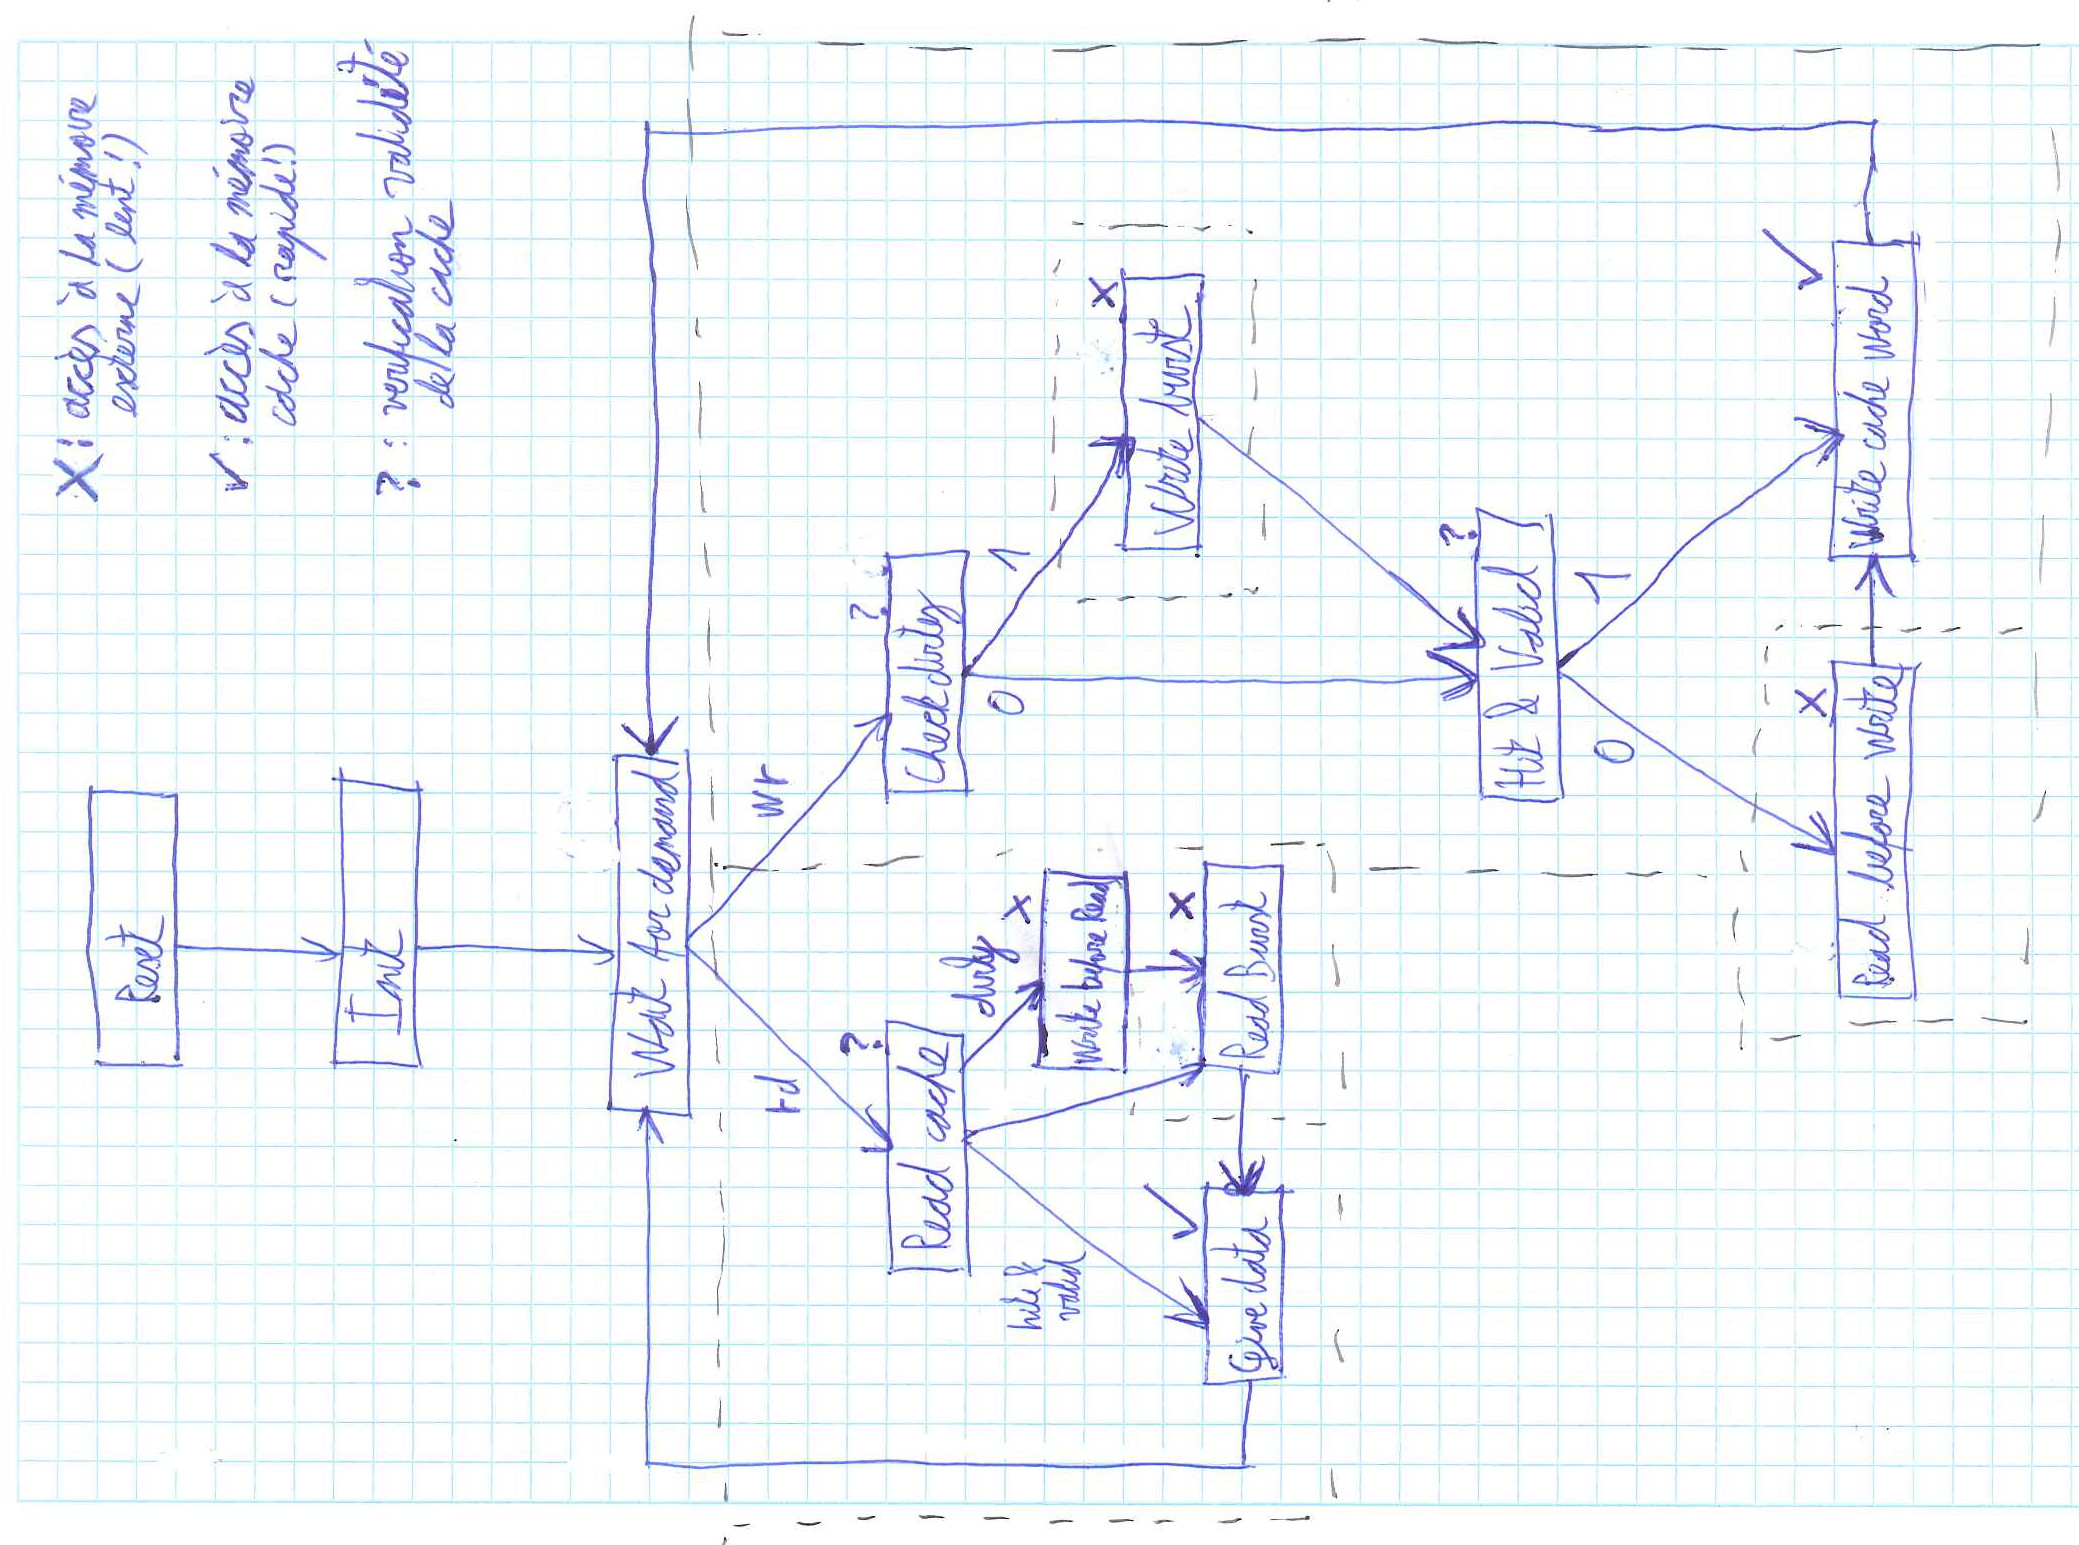
\includegraphics[width=1.3\textwidth, angle=-90]{images/mss}

\end{center}

\newpage

On commence tout d'abord par une initialisation des différents attributs de la cache. Il s'agit notamment de mettre les bits \texttt{valid} et \texttt{dirty} à 0 pour indiquer que la cache est vide et qu'elle doit donc être rempli.\\

Ensuite, dans \texttt{wait for demand}, on attend un signal de lecture ou écriture (\texttt{rd} ou \texttt{wr}). On est après redirigé dans la partie concerner.

\subsubsection{Lecture}
Pour la lecture, on vérifie d'abord s'il y a un hit. Pour cela, on vérifie si le tag trouvé via l'adresse correspond à celui en cache et que la ligne est valide.
Si la réponse est positive, on récupère directement la valeur dans la mémoire cache sinon, on doit chercher en mémoire d'abord.
L'accès en mémoire se fait à chaque fois en burst et de la manière suivante:

\begin{center}

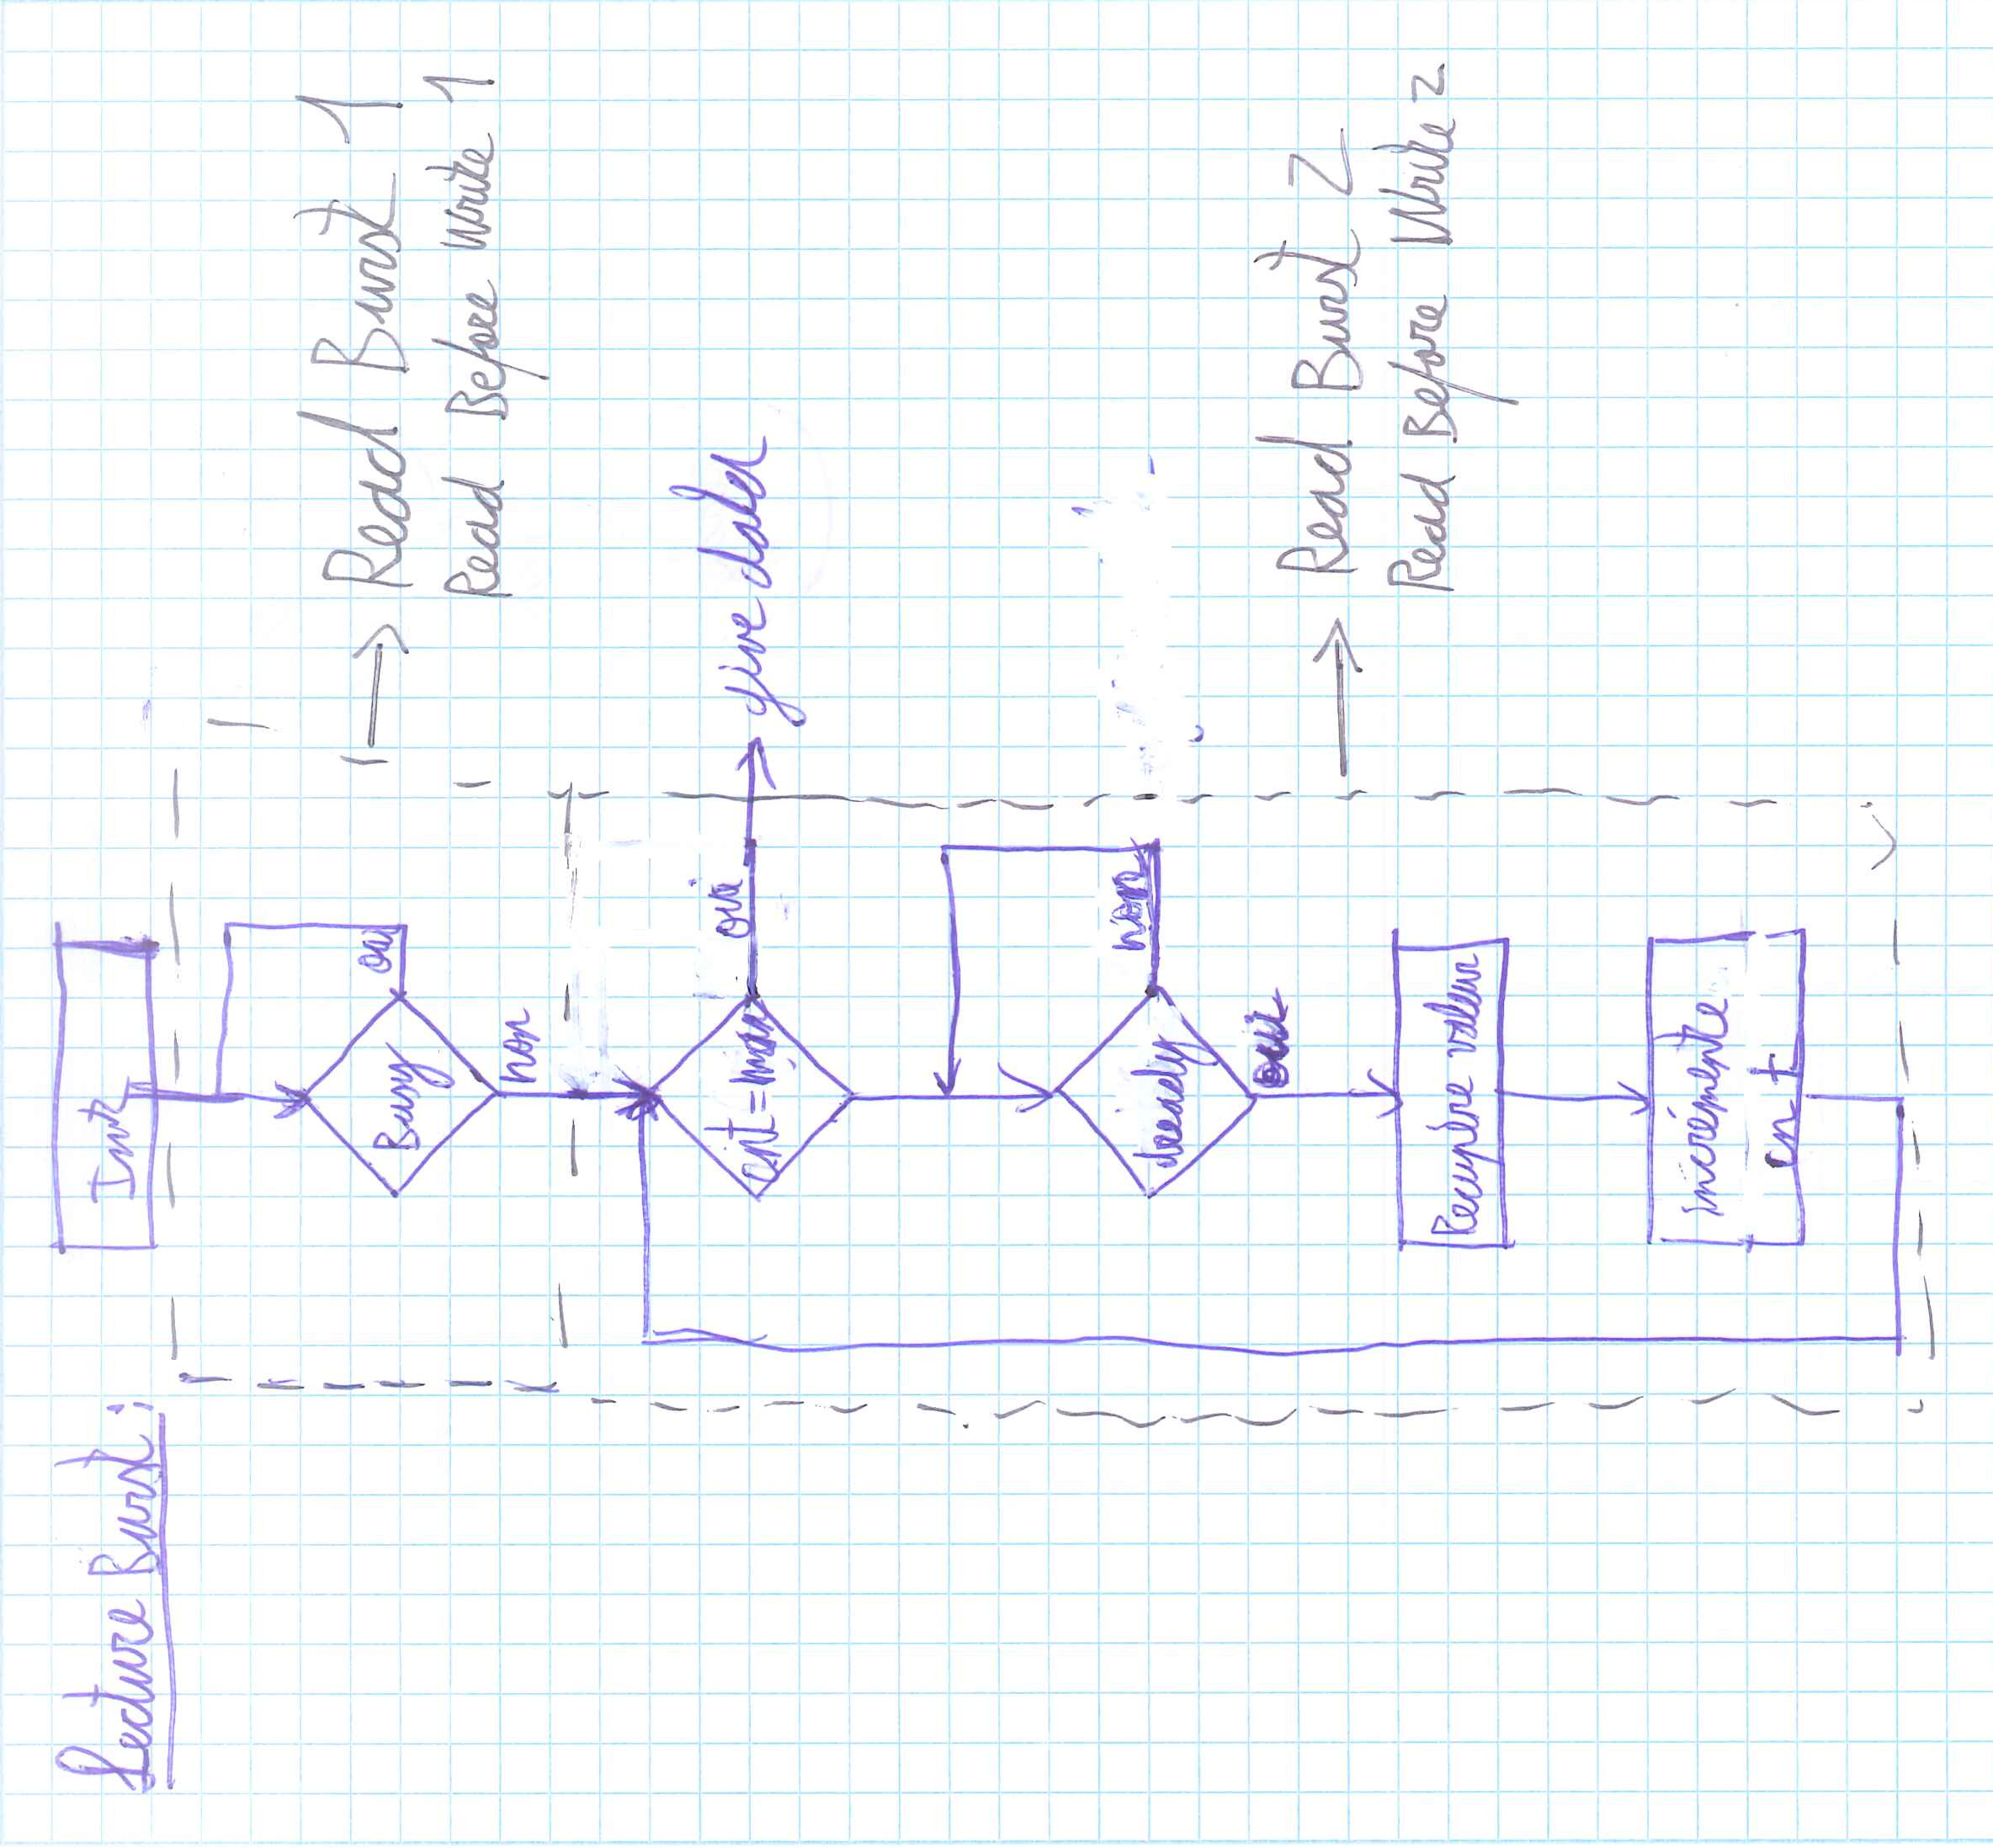
\includegraphics[width=0.7\textwidth, angle=-90]{images/mss_read}

\end{center}

On attend tout d'abord sur le busy car il se peut que la mémoire soit occupé lorsqu'on veut l’accéder. Une fois la mémoire libre, on lui demande les données, on vérifie qu'elles soit prêtent et les enregistres. On vérifie que la mémoire à finit le transfère via un compteur que l'on incrémente à chaque fois qu'une donnée a été récupérer avec succès.

\subsubsection{Écriture}
Pour l'écriture, on doit d'abord vérifier que la ligne à écrire contient le bon tag et dans le cas contraire qu'elle n'est pas \texttt{dirty}. Dans le cas où la réponse est négative, il faut écrire dans la mémoire pour la mettre à jour avant de changer le contenu de la cache car le bloque mémoire accédé sera différent.
L'écriture se fait en burst et se fait de la manière suivante:  
\begin{center}

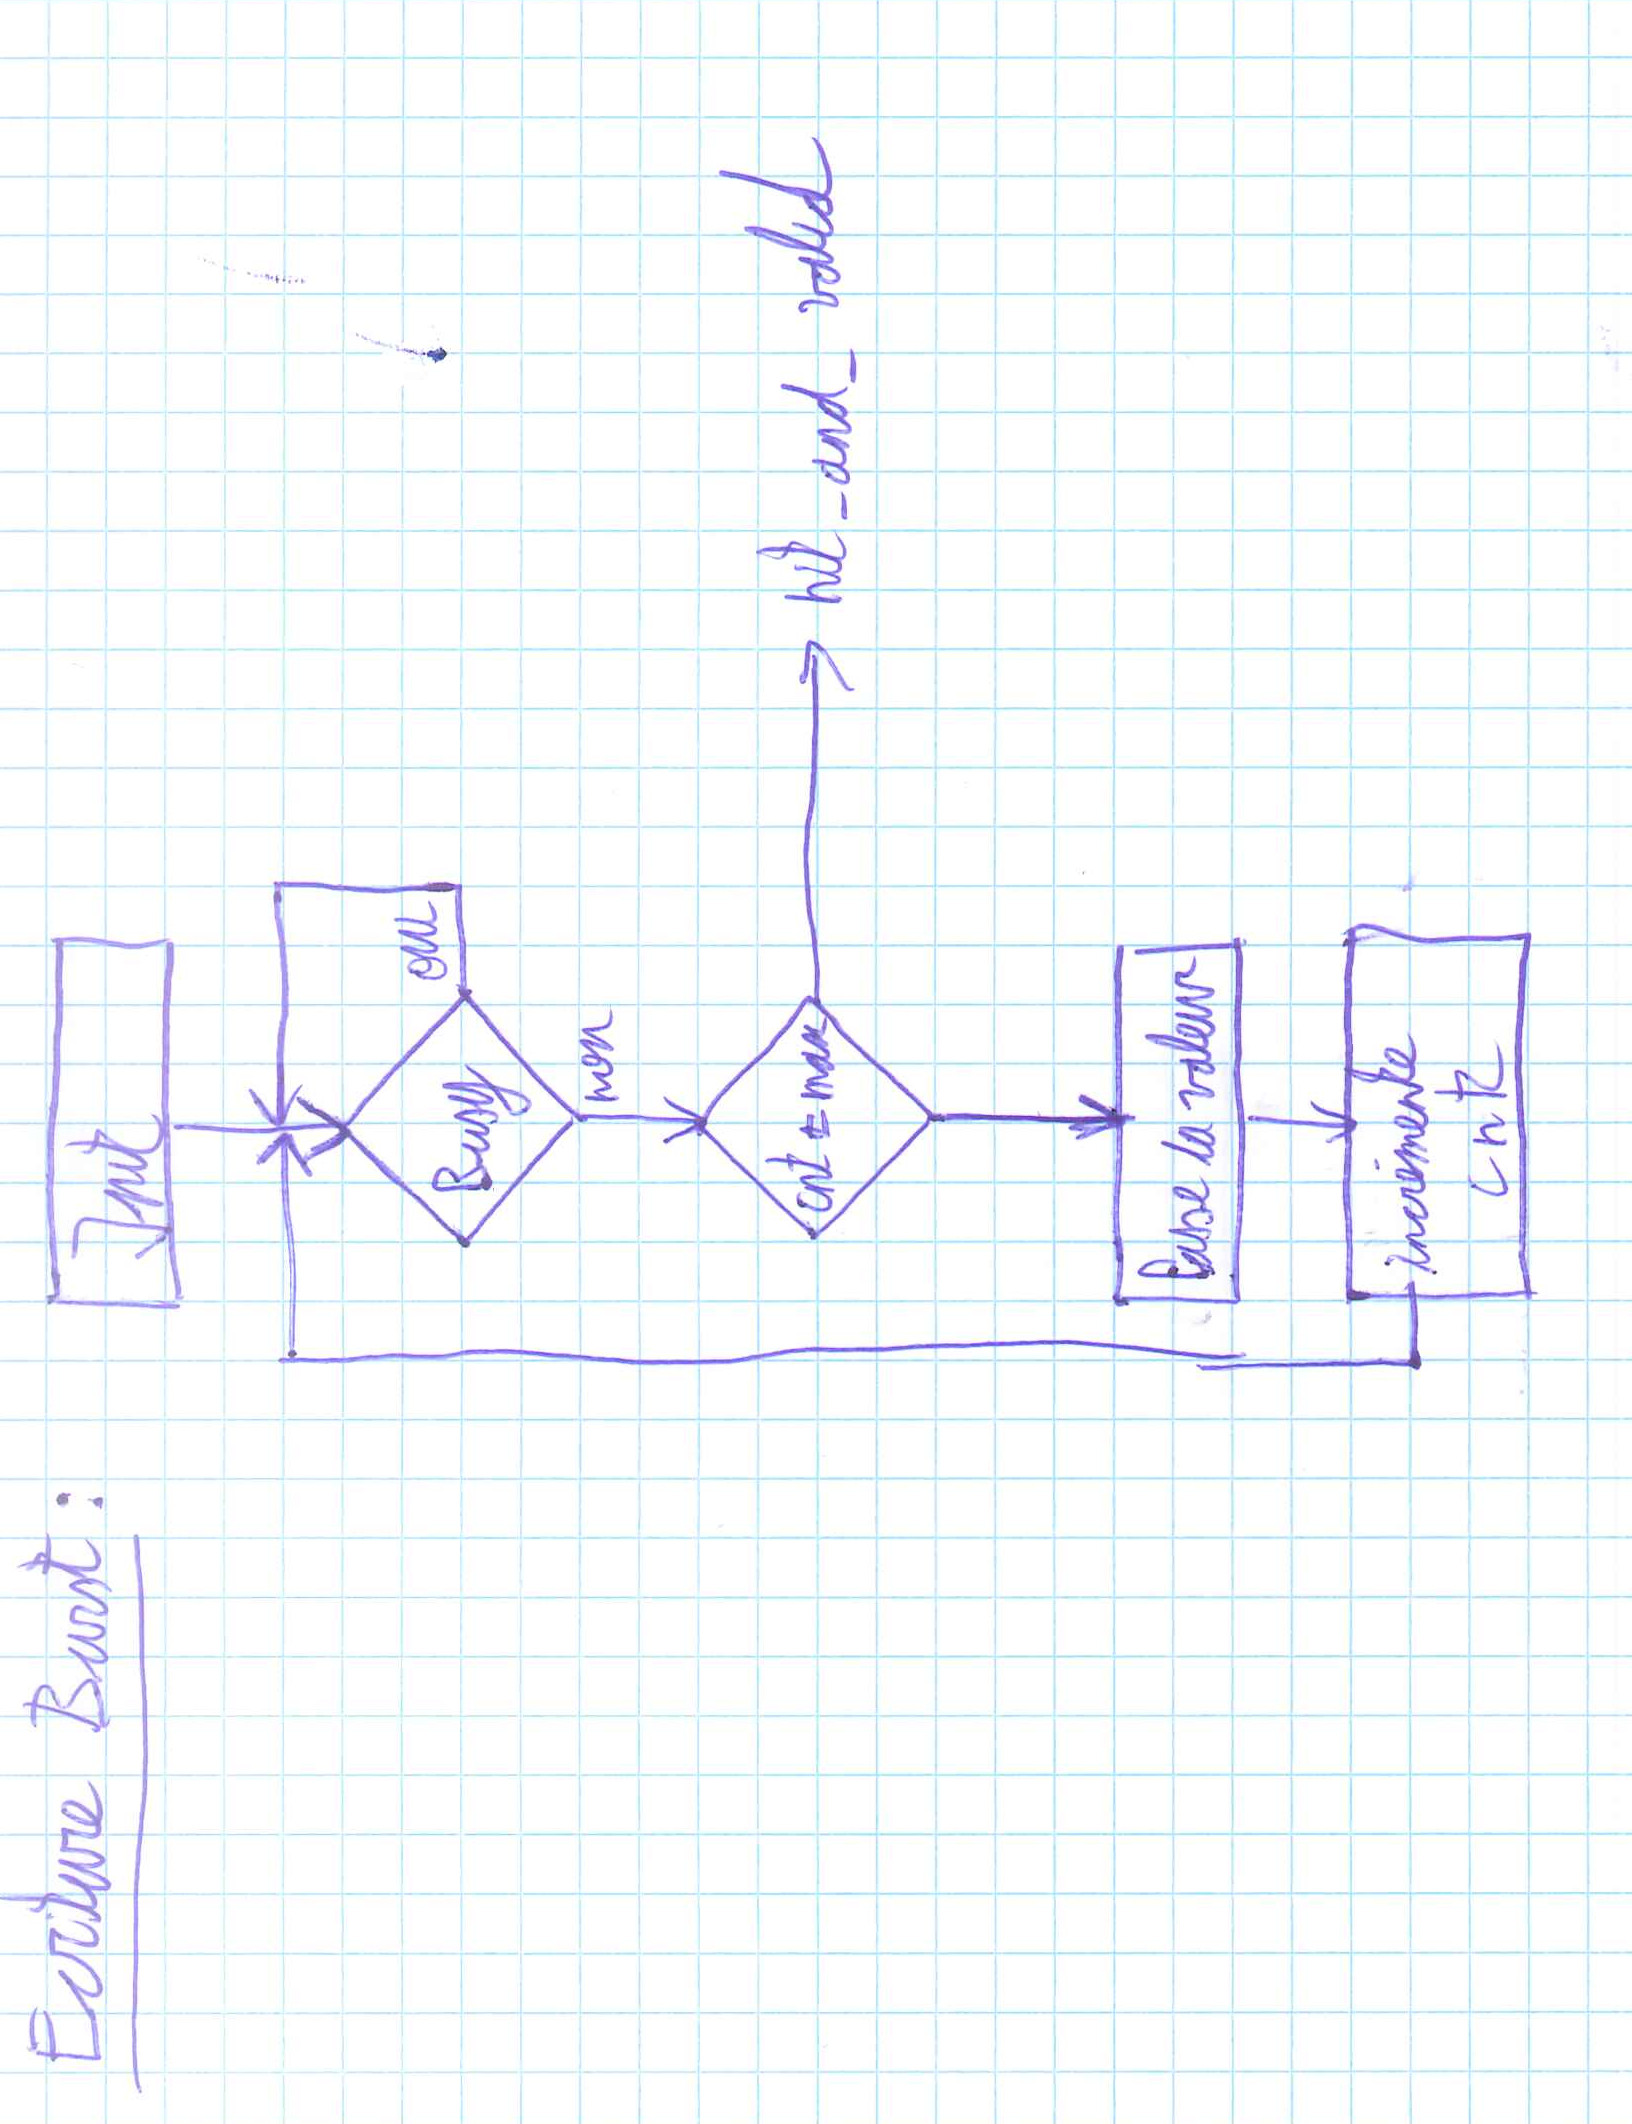
\includegraphics[width=0.5\textwidth, angle=-90]{images/mss_write}

\end{center}
Par rapport à la lecture, on n'attend toujours sur busy avant de passer la valeur.\\

Avant d'écrire en cache, on doit s’assurer que la ligne est valide. On évite ainsi d'écrire dans une ligne qui n'a pas de valeur cohérente par rapport à la mémoire, ce qui la fausserai plus tard dans l’exécution. Si la ligne est invalide, on fait une lecture en burst dans la mémoire. Une fois ceci fais, on modifie la valeur en cache et on met le bit \texttt{dirty} de la ligne à 1.

\section{Mémoire simulée}

\section{Conclusion}

\end{document}
